%---------------------------------------------------------
%	PACKAGES AND THEMES
%---------------------------------------------------------

% NOTE: This template and choice of fonts work only properly if compiled
% using XeLaTeX. On Overleaf, choose the compiler through the Menu in
% the top-left corner. Open the menu and the first setting is Compiler.
% It is probably at its default, pdfLaTeX


% https://ctan.math.utah.edu/ctan/tex-archive/macros/latex/contrib/beamer-contrib/themes/metropolis/doc/metropolistheme.pdf
\documentclass[aspectratio=169, 11pt]{beamer}

\usepackage{graphics, booktabs, makecell}
\usepackage{pgfplots}
\pgfplotsset{width=15cm,compat=1.13,
            every axis/.append style={
                    label style={font=\large} 
                    }}
\usepgfplotslibrary{external}
\usepackage{pgfplotstable}
\usetikzlibrary{patterns}

\usepackage{siunitx}
\sisetup{
        table-number-alignment=center,
        input-open-uncertainty  = ,
        input-close-uncertainty = ,
        table-align-text-pre    = false,
        table-align-text-post   = false,
        table-space-text-pre    = (
        }
        
\usepackage{tikz}
\usetikzlibrary{shapes,arrows,backgrounds,fit,positioning}
\tikzset{res/.style={ellipse,draw,minimum height=0.5cm,minimum width=0.8cm}}
\usepackage{multirow, hyperref}
\usepackage{wasysym}% Adds symbols

\usepackage{appendixnumberbeamer} % Restart number after appendix begins
\renewcommand{\appendixname}{\texorpdfstring{\translate{Appendix}}{Appendix}} % Because of bug

\usetheme[progressbar=foot, numbering=fraction]{metropolis}
%\setbeamertemplate{navigation symbols}{} % Removes the navigation symbols from the bottom of all slides

\definecolor{darkred}{rgb}{0.8,0,0}
\setbeamercolor{title separator}{fg=darkred}
\setbeamercolor{alerted text}{fg=orange}

\usepackage{graphicx} % Allows including images

% Define indicator ...
\DeclareSymbolFont{bbold}{U}{bbold}{m}{n}
\DeclareSymbolFontAlphabet{\mathbbold}{bbold}
\newcommand{\bi}{\mathbbold{1}}

% Deemphasize text
\newcommand{\light}{\textcolor{gray}}

\newcommand{\EE}{\mathbb{E}}
\newcommand{\PP}{\mathbb{P}}

\newcommand{\ToCslide}{\bgroup\setbeamertemplate{footline}{}% Hides slide counter
\addtocounter{framenumber}{-1}%
\begin{frame}{Outline}%
\tableofcontents%      Print ToC
\end{frame}\egroup}

%---------------------------------------------------------
%	TITLE PAGE
%---------------------------------------------------------

\title[Some title]{A title}

\author{Author names (comments are from Michela Giorcelli's presentation template in Western European History, 2019)}
\date{A date}

% Add bibliography
\usepackage[style=authoryear, maxcitenames=2, uniquelist=false, uniquename=false]{biblatex}
\addbibresource{References.bib}
\setbeamertemplate{bibliography item}{}

% Road map
\AtBeginSection[]{%
\bgroup\setbeamertemplate{footline}{}% Hides slide counter
\addtocounter{framenumber}{-1}%        Doesn't add to slide counter
\begin{frame}{Outline}%
\tableofcontents[currentsection]%      Print ToC
\end{frame}\egroup%
}

% Doesn't increases page counter after every pause
%\resetcounteronoverlays{page}

\begin{document}

\maketitle

{\metroset{sectionpage=none}%
\section{Introduction}}

\begin{frame}{Motivation}
    Observation 1
    
    Observation 2
    
    Observation 3
\end{frame}

\begin{frame}{Research question}
    \only<3->{\hypertarget{example_to_return_to1}{}}
    Main research question addressed with \alert{alerted} word!\pause
    
    Supplementary research question addressed\only<2->{\footnote{A footnote}}\pause
    
    Supplementary research question addressed \hyperlink{app_example}{\texttt{link text}~ \beamerskipbutton{To appendix}}
\end{frame}

\begin{frame}{This paper}
    Specific issue addressed
    
    How you think about the issue: Model\\
    \begin{itemize}
        \item ``Idea'' of model/theoretical framework
    \end{itemize}
    
    Method employed: Data\\
    \begin{itemize}
        \item ``Idea'' of identification
    \end{itemize}
\end{frame}

\begin{frame}{Relation to literature}
    \textbf{Motivating literature:} Paper 1, Paper 2
    
    Explain \emph{your} contribution w.r.t. the existing literature
    
    Do \emph{not} summarize others' papers
\end{frame}

\begin{frame}{Preview of findings}
    
\end{frame}

\ToCslide

\section{Model/setting}

\begin{frame}{Model}
    Give core idea of the model in words and figures
    
    Use the minimal number of Greek letters required to make your point\\
    \begin{itemize}
        \item But the model needs to be solved in the paper
    \end{itemize}
    
    Make clear what insights come out of the model and how this maps to what you will test in the data
    
    Your paper may prove the results for a large class of functions, but often the intuition is in a simpler case. Simplify!
    
    \small (If using someone's model, refer to it!)
\end{frame}

\begin{frame}{Setting}
    This section can also be about the empirical setting you exploit
    
    Give the audience enough information to understand it
    
    Do not provide too many details (include only what is relevant for the paper)
    
    Especially for papers outside US:\\
    \begin{itemize}
        \item Compare with the US
        \item Explain the differences
        \item Make an extra effort to explain why the setting is particularly good to answer the research question
    \end{itemize}
\end{frame}

\section{Data}

\begin{frame}{Data}
    What is the sample? What is the sampling frame?
    
    What is an observation in the dataset?
    
    Table 1: Summary statistics\\
    \begin{itemize}
        \item If needed, show balance across treatment and control
        \item Means and SDs of outcome variable
        \item Means and SDs of key regressors
    \end{itemize}
    
    Any weird data issues to be aware of? (E.g., attrition?)
\end{frame}

\section{Estimation}

\begin{frame}{Estimation}
    % Make nested itemize smaller
    \setbeamerfont*{itemize/enumerate body}{size=\fontsize{9}{8}}
    \setbeamerfont*{itemize/enumerate subbody}{parent=itemize/enumerate body}
    \setbeamerfont*{itemize/enumerate subsubbody}{parent=itemize/enumerate body}

    \small
    Empirical strategy\\
    \begin{itemize}
        \item Specification
        \begin{itemize}
            \item E.g., what regression; what moment condition
        \end{itemize}
        \item Identification assumption
        \begin{itemize}
            \item Should be in some measure of detail
            \item Should adhere to standard techniques
            \item A lot of seminars will get hung up here. \emph{Be very well prepared to defend specification}
        \end{itemize}
    \end{itemize}
    
    Estimation procedure\\
    \begin{itemize}
        \item Often will be trivial (OLS or other linear method)
        \item Sometimes more involved
    \end{itemize}
    
    Inference procedure\\
    \begin{itemize}
        \item Again, often trivial (clustered at location level)
        \item Sometimes more involved (wild clustered bootstrap)
    \end{itemize}
\end{frame}

\begin{frame}{A frame with math and a reference}
    Model \parencite{article1}
    \begin{equation}
    \begin{aligned}
        y_{i,g,t} &= \beta \times \text{treatment}_g \times \text{post}_t \\
        &\qquad + \delta_i + \eta_t + X_{i,t} + \varepsilon_{i,g,t}.
    \end{aligned}
    \end{equation}
    Another relevant citation is \cite{article2}
\end{frame}

\begin{frame}{A table}
    \footnotesize
    \setlength{\tabcolsep}{0.5em}
    \begin{center}
    \sisetup{table-format=-1.3, table-space-text-post={***}}
    \begin{tabular}{lSScSS}
    & \multicolumn{2}{c}{$\log y_1$} && 
      \multicolumn{2}{c}{$\log y_2$} \\
     \cmidrule{2-3}\cmidrule{5-6}
            & {(1)}     & {(2)}     && {(3)}     & {(4)}     \\ \midrule
    $\beta$
            & -0.214*** & -0.194*** &&  0.002    & -0.019    \\
            & (0.035)   & (0.029)   && (0.014)   & (0.014)   \\
    Other variable
            &  0.211*** &  0.222*** &&  0.135*** &  0.135*** \\
            & (0.035)   & (0.034)   && (0.032)   & (0.032)   \\ \midrule
    Observations 
            &  {11,308} & {19,666}  && {50,248}  & {85,048}  \\
    $R$-squared
            & {0.330}   & {0.374}   && {0.430}   & {0.437}   \\
    \end{tabular}%
    \end{center}
    
    Note: A note about the table above
\end{frame}

\section{Additional sections/extensions}

\begin{frame}
    This section can include lots of things
    
    \begin{itemize}
        \item Theoretical/model
        \item Empirical
        \begin{itemize}
            \item Robustness checks
            \item Overidentification tests
            \item Welfare computations
            \item Counterfactuals
        \end{itemize}
    \end{itemize}
\end{frame}

\section{Conclusion}

\begin{frame}{Conclusions}
    Reiterate what we learned
    
    A new research or policy question the work raises, that we could not anticipate without having done the work of reading the paper/listening to the talk
\end{frame}

\begin{frame}[plain, noframenumbering]
    \begin{center}
        \LARGE Thanks, the end, etc.
    \end{center}
\end{frame}

\AtBeginSection[]{}

\appendix

\section{References}

\begin{frame}[allowframebreaks]{References}
\begin{scriptsize}
    \printbibliography
\end{scriptsize}
\end{frame}

\section{Appendix}

% Appendix road map
\AtBeginSection[]{%
\begin{frame}{Appendix}
\tableofcontents[currentsection] %
\end{frame}%
}

\section{Extra: Appendix}

\begin{frame}{An appendix frame}
    With a Tikz graph!
    
    \begin{center}
    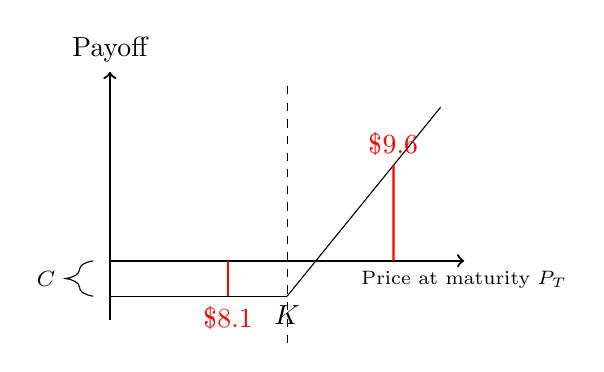
\begin{tikzpicture}[scale=1.5]
    % Draw axes
    \draw [<->,thick] (0,1.6) node (yaxis) [above] {Payoff}
        |- (3,0) node (xaxis) [below] {\scriptsize Price at maturity $P_T$};
    \draw [thick] (0,0) -- (0, -.5);
    
    \draw (0,-.3) -- (1.5,-.3) coordinate (K);
    \draw (K) node[below] {$K$} -- (2.8,1.3) coordinate (U);

    \draw [dashed] (1.5,-.7) -- (1.5, 1.5);
    
    \draw [decorate,decoration={brace,amplitude=10pt},xshift=-4pt,yshift=0pt]
    (0,-.3) -- (0,0) node [black,midway,xshift=-0.6cm] 
    {\footnotesize $C$};
    
    \coordinate (p_u)  at (2.4, 0);
    \coordinate (p_uu) at (2.4, 1);
    \coordinate (c) at (intersection of K--U and p_u--p_uu);
    
    \pause
    \draw [thick, red] (p_u) -- (c) node[above] {\$9.6};
    
    \pause
    \draw [thick, red] (1,0) -- (1,-0.3) node[below] {\$8.1};
    
    \end{tikzpicture}
    \end{center}
\end{frame}

\section{Appendix, part 2}

\begin{frame}[label=app_example]{Another appendix frame}
    With two different buttons that takes us back to the original page \quad \hyperlink{example_to_return_to1}{\beamerskipbutton{Go back}}\quad\hyperlink{example_to_return_to1}{\beamerbutton{Jump to}}
\end{frame}

\end{document}
